\newcommand\tab[1][1cm]{\hspace*{#1}}

\chapter{Fonctionnalités}
\label{s:fonctionnalite}

\section{Image}
\subsection{Importation}
Non implémenté

\subsection{Exportation}
L'exportation en image est implémentée grâce à la méthode imageExport de la classe renderer. Tout d’abord, on dessine la scène, sans l’interface graphique. Ensuite, on sauvegarde une capture de l’écran avec le nom, un «time stamp», pour que le fichier soit unique, et l’extension reçue en paramètre.\\

\begin{lstlisting}
void renderer::imageExport(const string name, const string extension)
{
	draw();
	
	ofImage imageTemp;
	
	string timestamp = ofGetTimestampString("-%y%m%d-%H%M%S-%i");
	
	string fileName = name + timestamp + "." + extension;
	
	imageTemp.grabScreen(0, 0, ofGetWindowWidth(), ofGetWindowHeight());
	
	imageTemp.save(fileName);
	
	ofLog() << "<export image: " << fileName << ">";
}
\end{lstlisting}


\subsection{Espace de couleur}
 L'espace de couleur utilisé par l'application est le HSB. Ainsi, pour chaque couleur à saisir, trois «sliders» sont disposés dans l'interface pour saisir la teinte (Hue), la saturation (Saturation) et la valeur (Brightess).\\
 
 En soi, à chaque mise à jour de l'application, l'application met à jour les valeurs des attributs de couleur dans la classe renderer. Ainsi, à chaque instant, le renderer a les couleurs entrées par l'utilisateur.\\
 
 Voici un exemple d'initiation des valeurs pour la couleur de remplissage:
 \begin{lstlisting}
 	fillHue.setName("Teinte");
 	fillHue.setMin(0);
 	fillHue.setMax(255);
 	fillHue.set(0);
 
 	fillSaturation.setName("Saturation");
 	fillSaturation.setMin(0);
 	fillSaturation.setMax(255);
 	fillSaturation.set(100);
 
 	fillBrightess.setName("Valeur");
 	fillBrightess.setMin(0);
	fillBrightess.setMax(255);
	fillBrightess.set(255);
 
 	fillAlpha.setName("Transparence");
 	fillAlpha.setMin(0);
 	fillAlpha.setMax(255);
 	fillAlpha.set(255);
 \end{lstlisting} 

Voici la méthode qui génère les couleurs à partir de l'espace HSB:
\begin{lstlisting}
	void ofApp::setColors()
	{
		stroke = ofColor::fromHsb(strokeHue, strokeSaturation, strokeBrightess, strokeAlpha);
		fill = ofColor::fromHsb(fillHue, fillSaturation, fillBrightess, fillAlpha);
		background = ofColor::fromHsb(bgHue, bgSaturation, bgBrightess);
	}
\end{lstlisting} 

Voici la méthode qui met à jour les couleurs du renderer (et l'épaisseur de lignes):
\begin{lstlisting}
	void ofApp::setRendererParameter() {
		
		rend->stroke = stroke;
		rend->fill = fill;
		rend->background = background;
		
		rend->strokeThickness = strokeThickness;
	}
\end{lstlisting}


\subsection{Traitement d'image}
Une catégorie située au coin droit de l’écran permet l’utilisation de plusieurs filtres s’affichant sur l’entièreté de la scène. Elle regroupe trois types de filtres: le brouillage, l’inversion des couleurs et la dilatation. Les trois filtres peuvent être appliqués tous en même temps ou un à la fois.\\

Un objet ofxCvColorImage est utilisé pour la réalisation des filtres. On capture les pixels de la scène et on l’ajoute dans cet objet, pour ensuite lui faire subir les filtres sélectionnés par l’utilisateur. Les fonctions blur(), invert() et dilate() ont été utilisées pour construire le filtre. Ces fonctions utilisent différentes opérations sur chaque pixel de l’image pour les modifier.\\

Voici une image d’une scène avec des filtres d’inversement de couleurs et de brouillage:\\
\begin{figure}[h]
	\centering
	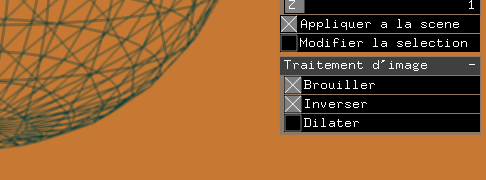
\includegraphics[width=5cm]{fig/filters.png}
	\caption{Une scène avec filtres.}
	\label{fig:filtres}
\end{figure}


\subsection{Image procédurale}
Non implémenté

\newpage

\section{Dessin vectoriel}

\subsection{Curseur dynamique}

Dans notre application il y a une interface graphique créée avec ofxGui. Cette technologie, malgré le fait qu'elle soit très pratique pour nos besoins, contient des boutons, des cases à cocher, des "sliders", des groupes, mais le curseur était toujours identique (en forme de flèche), ce qui ne rendait pas évident avec quoi on peut ou ne peut pas interagir.

Nous avons donc ajouté, en utilisant les événements mouseMoved() de notre fenêtre et des différents contrôles, une modification dynamique du curseur selon au-dessus de quoi il se trouve.

Au a donc trois curseurs différents.

Le curseur normal, qui est présent quand la souris est dans l'espace de dessin

\begin{figure}[h]
	\centering
	\includegraphics[width=5cm]{fig/curseurNormal.png}
	\caption{Curseur normal de type "flèche"}
	\label{fig:curseurNormal}
\end{figure}

Le curseur de type "main", qui est présent quand la souris est au-dessus d'un bouton ou d'une case à cocher

\begin{figure}[h]
	\centering
	\includegraphics[width=5cm]{fig/curseurBouton.png}
	\caption{Curseur pour bouton de type "main"}
	\label{fig:curseurBouton}
\end{figure}

Et le curseur de type "slider", qui est présent quand la souris est au-dessus d'un contrôle du même nom.

\begin{figure}[h]
	\centering
	\includegraphics[width=5cm]{fig/curseurSlider.png}
	\caption{Curseur slider de type "slider"}
	\label{fig:curseurSlider}
\end{figure}

\begin{lstlisting}
void ofApp::mouseMoved(int x, int y) {
	HCURSOR curs;
	if (!cursorIsInControl(x, y))
	{
		curs = LoadCursor(NULL, IDC_ARROW);
		SetCursor(curs);
	}
}
\end{lstlisting}

\begin{lstlisting}
bool ofxButton::mouseMoved(ofMouseEventArgs & args){

	HCURSOR curs;
	if (cursorIsInControl(args.x, args.y))
	{
		curs = LoadCursor(NULL, IDC_HAND);
		SetCursor(curs);
	}
	return ofxToggle::mouseMoved(args);
}
\end{lstlisting}

\begin{lstlisting}
template<typename Type>
bool ofxSlider<Type>::mouseMoved(ofMouseEventArgs & args){
	mouseInside = isGuiDrawing() && b.inside(ofPoint(args.x,args.y));
	
	HCURSOR curs;
	if (mouseInside)
	{
		curs = LoadCursor(NULL, IDC_SIZEWE);
		SetCursor(curs);
	}
	
	return mouseInside;
}
\end{lstlisting}

\subsection{Primitives vectorielles}

Dans les types de primitives disponibles, on trouve la catégorie 2D. En sélectionnant cette catégorie, on peut ainsi dessiner des carrés, des cercles (ellipses), des triangles, des lignes et des points. Toutes ces primitives sont affectées par la position, la taille, l’épaisseur de traits, la couleur de remplissage et de bordure ainsi que la texture passée par l’utilisateur.\\

Des objets ofPath sont utilisés pour tous les types de primitives 2D créés. Afin d’avoir une meilleure intégration à la scène, une casse générique de primitives 2D a été créée. Pour les différents types, différentes méthodes ont été conçues pour créer les primitives. Ces méthodes utilisent les méthodes ellipse(), circle(), rect(), triangle() et line(). Elles appliquent chaque propriété spécifiée par l’utilisateur. Après chaque ajout, on ajoute ensuite les primitives dans la scène.\\

Voici à quoi ressemblent les différentes primitives 2D:\\
\begin{figure}[h]
	\centering
	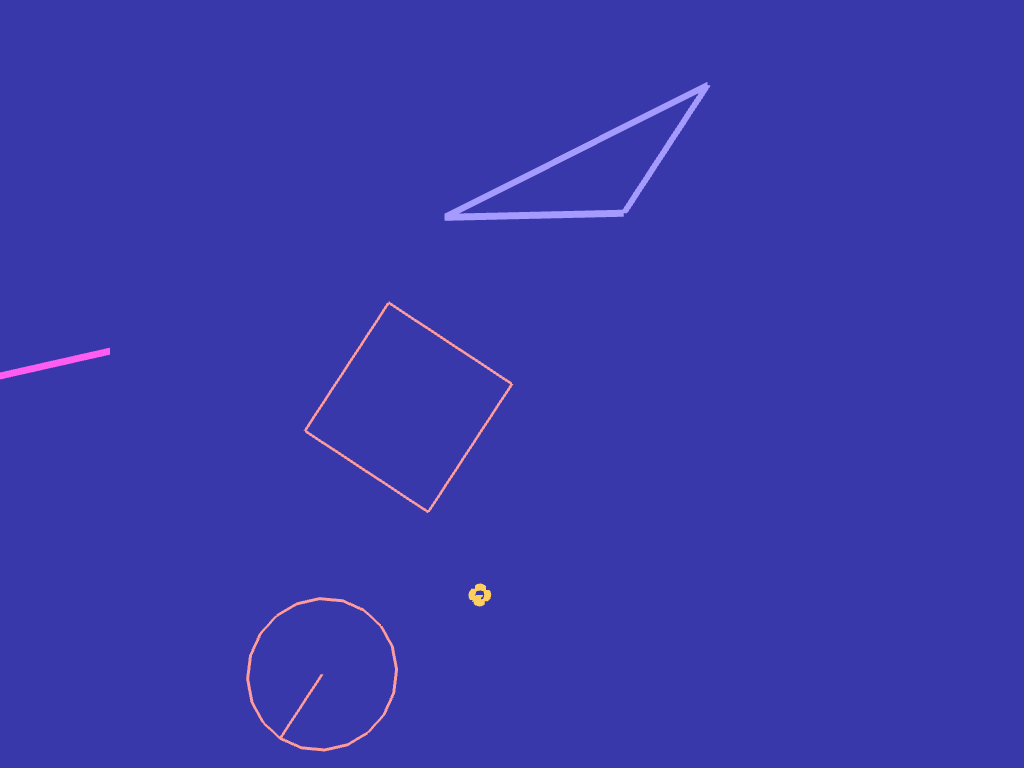
\includegraphics[width=5cm]{fig/primitives2d.png}
	\caption{Une scène avec primitives 2D.}
	\label{fig:prim2D}
\end{figure}

\subsection{Formes vectorielles}
La forme qui a été implémentée est un cornet de crème glacée, formé d'un cône et d'une sphère. Le code se trouve dans «renderer::createIceCream()» 

\begin{lstlisting}
ofParameter<bool>  renderer::createIcecream(int x, int y, int z, int sizeX, int sizeY, int sizeZ, ofColor color) {
	ofSpherePrimitive* ball = new ofSpherePrimitive();
	ball->setPosition(x, y + sizeY / 3, z);
	
	ofConePrimitive* cone = new ofConePrimitive();
	cone->setPosition(x, y - sizeY / 3, z);
	
	float smallestSphere = min(sizeX, min(sizeY, sizeZ));
	ball->setRadius(smallestSphere / 2);
	
	float smallestCone = min(sizeX, sizeZ);
	cone->setRadius(smallestCone / 2);
	cone->setHeight(sizeY);
	
	float newX = (float)sizeX / smallestSphere;
	float newY = (float)sizeY / smallestSphere;
	float newZ = (float)sizeZ / smallestSphere;
	
	ofMatrix4x4 matrix = ofMatrix4x4();
	matrix.scale(newX, newY, newZ);
	matrix.setTranslation(x, y, z);
	
	forme3d forme{ ball, color, matrix };
	forme.addPrimitive(cone);
	forme.setName("IceCream " + to_string(scn->nbElements() + 1));
	scn->addElement(forme);
	return forme.selected;
}
\end{lstlisting}

\begin{figure}[h]
	\centering
	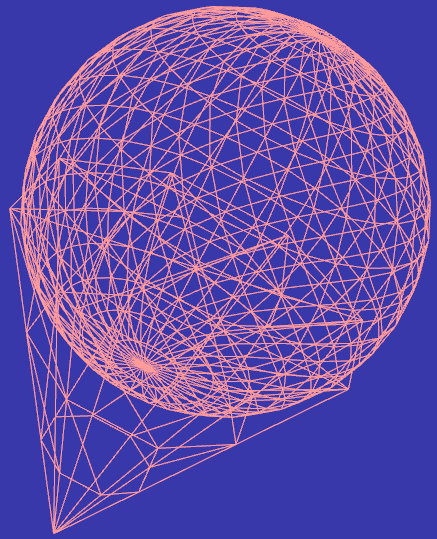
\includegraphics[width=5cm]{fig/iceCream.png}
	\caption{Cornet de crème glacée!}
	\label{fig:iceCream}
\end{figure}

On aurait bien voulu le faire avec des primitives 2D, mais on s'est dit qu'en 3D ça amenait un peu plus de défi!

\subsection{Outils de dessin}
L'outil de dessin a été implémenté en ajoutant des «sliders» dans l'interface afin de pouvoir modifier la couleur de remplissage, la couleur du contour, la couleur d'arrière-plan et l'épaisseur des lignes de contour. Ainsi, il possible de modifier en tout temps la couleur d'arrière-plan ou bien de modifier la couleur de remplissage, la couleur de contour et l'épaisseur des lignes de contour pour la création de primitive.\\

En pratique, à chaque mise à jour de l'application, les valeurs des attributs de la classe renderer sont mises à jour. Ainsi, les valeurs de couleurs ou d'épaisseur des lignes sont à jour lors de la création d'une primitive, tout comme la couleur d'arrière-plan est à jour lorsque l'arrière-plan est redessiné. \\ 

Voici la méthode qui met à jour les couleurs et l'épaisseur de lignes du renderer:
\begin{lstlisting}
	void ofApp::setRendererParameter() {
		
		rend->stroke = stroke;
		rend->fill = fill;
		rend->background = background;
		
		rend->strokeThickness = strokeThickness;
	}
\end{lstlisting}

Voici la méthode qui affiche à l'écran le contenu du renderer. La première ligne consiste à dessiner l'arrière-plan:
\begin{lstlisting}
	void renderer::draw()
	{
		ofClear(background);
		
		[...]
	}
\end{lstlisting}

Voici une des méthodes qui ajoute une primitives à la scène. Les paramètres «fill» et «stroke» utilisés ici sont les attributs de couleurs de remplissage et de contour de la classe renderer:
\begin{lstlisting}
	ofParameter<bool> renderer::createSquare(float x, float y, float w, float h) {
		return createSquare(x,y,w,h,fill, stroke);
	}
\end{lstlisting}

\subsection{Interface}
L'application est dotée d'une interface utilisateur qui permet de modifier les paramètres d'une primitive à ajouter, ajouter une primitive à la scène, vider la scène, modifier les paramètres de la caméra, appliquer des transformations sur les primitives ou sur la scène, appliquer des effets de traitement d'image, sélectionner des primitives à l'aide d'une liste à cocher, importer un modèle 3D, exporter en image et quitter. \\

L'interface a été développée avec l'extension ofxGui. Ainsi, nous avons créé des «panels» (ofxPanel) dans lesquels les différents paramètres de l'application ont été ajoutés et l'extension se charge de générer les «sliders» et les cases à cocher associées aux paramètres. Nous avons aussi pu ajouter des boutons (ofxButton).\\

Comme l'essentiel du code de la classe qui gère l'interface représente plus de 1000 lignes, seulement quelques exemples seront montrés afin d'alléger ce document.\\

Voici l'initialisation de paramètres:
\begin{lstlisting}
void ofApp::initOfParameters() 
{
	[...]
	
	primPosX.setName("X");
	primPosX.setMin(MinX);
	primPosX.setMax(MaxX);
	primPosX.set((MinX + MaxX) / 2);
	
	primPosY.setName("Y");
	primPosY.setMin(MinY);
	primPosY.setMax(MaxY);
	primPosY.set((MinY + MaxY) / 2);
	
	primPosZ.setName("Z");
	primPosZ.setMin(MinZ);
	primPosZ.setMax(MaxZ);
	primPosZ.set((MinZ + MaxZ) / 2);
	
	[...]
}
\end{lstlisting}

Voici l'initialisation de groupes de paramètres (ofParameterGroup):
\begin{lstlisting}
void ofApp::initGroups()
{
	[...]
	
	groupPrimitivePosition2D.setName("Position");
	groupPrimitivePosition2D.add(primPosX.set(primPosX));
	groupPrimitivePosition2D.add(primPosY.set(primPosY));
	
	groupPrimitivePosition3D.setName("Position");
	groupPrimitivePosition3D.add(primPosX.set(primPosX));
	groupPrimitivePosition3D.add(primPosY.set(primPosY));
	groupPrimitivePosition3D.add(primPosZ.set(primPosZ));
	
	[...]
}
\end{lstlisting}

Voici la configuration de menu:
\begin{lstlisting}
void ofApp::setupMenu2D() {

	menu2D.setDefaultWidth(200);
	
	menu2D.setup();
	
	menu2D.add(groupPrimitiveType2D);
	menu2D.add(groupPrimitivePosition2D);
	menu2D.add(groupPrimitiveSize2D);
	
	menu2D.add(groupThick);
	
	menu2D.add(groupFill);
	
	menu2D.add(groupStroke);
	
	menu2D.add(groupTexture);
	
	menu2D.minimizeAll();
	
	menu2D.registerMouseEvents();
}
\end{lstlisting}

Voici la configuration des écouteurs sur les différents boutons de l'application:
\begin{lstlisting}
void ofApp::initButtonListener() {
	btnDrawPrimitive.addListener(this, &ofApp::btnDrawPrimitiveClicked);
	btnClear.addListener(this, &ofApp::btnClearClicked);
	btnExit.addListener(this, &ofApp::btnExitClicked);
	
	btnExport.addListener(this, &ofApp::btnExportClicked);
	btnImport.addListener(this, &ofApp::btnImportClicked);
	
	btnApplySelect.addListener(this, &ofApp::btnApplySelectClicked);

\end{lstlisting}

Voici la méthode setup de la classe ofApp:
\begin{lstlisting}
void ofApp::setup()
{
	[...]
	
	initOfParameters();
	initGroups();
	
	setupMenu2D();
	setupMenu3D();
	setupCameraMenu();
	setupTransformationMenu();
	setupOptionMenu();
	setupSelectionMenu();
	
	initButtonListener();
	
	[...]
}
\end{lstlisting}

Voici une capture d'écran pour montrer l'interface:
\begin{figure}[h]
	\centering
	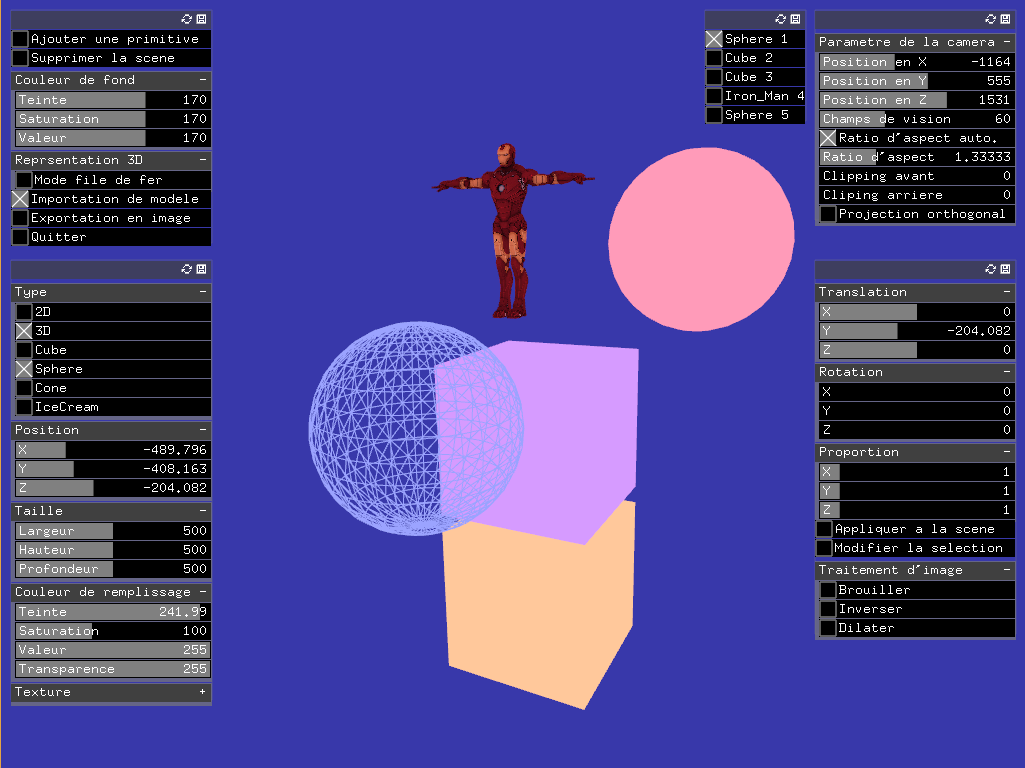
\includegraphics[width=15cm]{fig/InterfaceComplet.png}
	\caption{Exemple d'interface}
	\label{fig:interface}
\end{figure}

\pagebreak
\section{Transformation}
\subsection{Transformation interactive}
Une catégorie à droite de l’application permet de transformer le système de coordonnées des entités géométriques de la scène. On peut exercer des transformations telles que la translation en X, Y et Z, la rotation en X, Y et Z ainsi que la proportion en X, Y et Z. Elle peut se faire autant en temps réel qu’en différé. \\

Les matrices de transformation d’openframeworks sont utilisées pour la réalisation des transformations. On utilise les méthodes ofPushMatrix() et ofPopMatrix(). Une fois la matrice empilée, on ajoute les transformations à l’aide des méthodes ofTranslate(), ofRotate() et ofScale() selon les paramètres inscrits par l’utilisateur. Enfin, on dépile la matrice pour permettre la transformation.\\

Voici le menu des transformations et ces différentes options:\\
\begin{figure}[h]
	\centering
	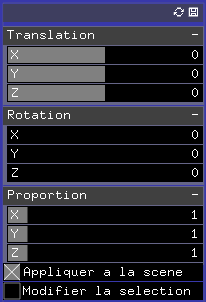
\includegraphics[width=5cm]{fig/transformations.png}
	\caption{Menu des transformations.}
	\label{fig:transformations}
\end{figure}

\subsection{Structure de scène}
La structure de scène a été implémentée sous la forme d'un arbre ordonné, dans lequel les feuilles sont les éléments de la scène. La classe scène comprend 4 classes interne, soit «element», «group», «node» et «scene\_iterator». Les classes «group» et «node» héritent d'«element» et  servent à stocker tout ce qui se trouve dans la scène. La classe «scene\_iterator» permet, quant à elle, de parcourir les éléments pour les dessiner. \\

On utilise les «shared\_ptr» au lieu des pointeurs normaux pour conserver les éléments qui sont ajoutés à la scène pour ne pas avoir à trop gérer la mémoire.\\

L'essentiel du code de la scène se trouve dans les méthodes addElement de la scène, des sous-classes de stockage et l'operator++ de l'itérateur.\\

\begin{lstlisting}
void scene::addElement(size_t index, primitive_ptr& p, bool insertFirstChild) {
	if (index == 0 && !insertFirstChild {
		throw invalid_argument("root don't have parent...");
	}
	root->addElement(index, p, insertFirstChild);
}

//Retourne la quantite d'element ajoute
size_t scene::node::addElement(size_t index, primitive_ptr& p, bool insertFirstChild) {
	if (index != this->index) {
		throw invalid_argument("index need to be equals to the index of the node");
	}
	if (insertFirstChild) {
		throw invalid_argument("node need to be wraped in a group");
	}
	this->content = p;
	contentType = "primitive";
	return 1;
}

//Retourne la quantite d'element ajoute
size_t scene::group::addElement(size_t index, primitive_ptr& p, bool insertFirstChild) {
	size_t addedSize = 0;
	
	if (this->index == index) {
		if (insertFirstChild) {
			//Inserer comme premier element
			childrens.insert(childrens.begin(), element_ptr{ new node{ index + 1, height + 1, p } });
			for (auto& it = childrens.begin() + 1; it < childrens.end(); ++it) {
				it->get()->setIndex(it->get()->getIndex() + 1);
			}
			addedSize++;
		} else {
			throw invalid_argument("element must to be add in the parent");
		}
	} else {
		size_t ubound = childrens.size();
		size_t lbound = 0;
		size_t i;
		
		//Recherche binaire
		while (lbound <= ubound) {
			i = lbound + (ubound - lbound) / 2;
			if (childrens[i]->getIndex() == index) {
				if (insertFirstChild) {
					if (childrens[i]->getType() != "group") {
						group_ptr temp = group_ptr{ new group{ index, height + 1 } };
						temp->childrens.push_back(childrens[i]);
						temp->childrens[0]->setIndex(index + 1);
						temp->childrens[0]->setHeight(height + 2);
						temp->size = temp->childrens[0]->getSize() + 1;
						childrens[i] = temp;
						addedSize++;
					}
					addedSize += childrens[i]->addElement(index, p, insertFirstChild);
				} else {
					childrens.insert(childrens.begin() + i + 1, element_ptr{ new node{ index + childrens[i]->getSize(), height + 1, p } });
					i++;
					addedSize++;
				}
				i++;
				break;
			} else if (childrens[i]->getIndex() < index) {
				lbound = i + 1;
				if (ubound < lbound) {
					//Ajoute l'element dans le groupe sous-jacent
					addedSize += childrens[i]->addElement(index, p, insertFirstChild);
					i++;
					break;
				}
			} else {
				ubound = i - 1;
				if (ubound < lbound) {
					//Ajoute l'element dans le groupe sous-jacent
					addedSize += childrens[i - 1]->addElement(index, p, insertFirstChild);
					break;
				}
			}
		}	
		for (auto& it = childrens.begin() + i; it < childrens.end(); ++it) {
			it->get()->setIndex(it->get()->getIndex() + addedSize);
		}
	}
	size += addedSize;
	return addedSize;
}

//Avance jusqu'au prochain node
void scene::scene_iterator::operator++() {
	for (rootIndex; rootIndex <= root->getSize(); ++rootIndex) {
		element* elem = root->getElement(rootIndex);
		if (elem->getType() != "group" && elem->getType() != "root") {
			primitive_ptr ptr = (dynamic_cast<node*>(elem))->content;
			if (p != ptr) {
				p = ptr;
				break;
			}
		}
	}
	if (rootIndex > root->getSize()) {
		p = primitive_ptr{ nullptr };
	}
}
\end{lstlisting}
Comme vous avez sans doute remarqué, l'ajout d'élément à la scène se fait récursivement, à l'index en paramètre. Le paramètre «insertFirstChild» indique s'il faut insérer l'élément comme le premier enfant de l'élément à l'index en paramètre. S'il est faux, on insère simplement le nouvel élément après l'index. Dans group::addElement, on utilise un algorithme de recherche binaire pour trouver dans ou après quel élément il faut ajouter le nouvel élément. L'operator++, quant à lui, parcours la scène en s'arrêtant seulement sur les classes node. \\

Malheureusement, par manque de temps la structure de scène n'est pas utilisée à son plein potentiel et tous les éléments sont stockés dans le groupe à la racine de la scène. Il est tout de même possible de voir le résultat en changeant la ligne «\#define test 0» pour «\#define test 1» dans le fichier «main.cpp». Vous verrez alors le résultat de l'exécution des tests de la classe «scene» (principalement de l'ajout et de la suppression d'élément), se trouvant à la fin de «scene.cpp». \\

\newpage

\subsection{Sélection multiple}

Dans notre application, toutes les entités géométriques, soit les primitives en 2D, les primitives en 3D et les modèles 3D importés du disque, apparaissent dans un menu avec un nom unique.

\begin{figure}[h]
	\centering
	\includegraphics[width=5cm]{fig/menuSelection.png}
	\caption{Menu de sélection}
	\label{fig:menuSelection}
\end{figure}

À partir de là, il est possible d'en sélectionner un ou plusieurs.

\begin{figure}[h]
	\centering
	\includegraphics[width=5cm]{fig/menuSelectionPlusieurs.png}
	\caption{Plusieurs entités sélectionnées}
	\label{fig:selectionMultiple}
\end{figure}

\newpage

Lorsqu'on n'est pas en mode «wireframe», les entités sélectionnées seront affichées en «wireframe» quand même, de façon à les identifier. Comme le mode «wireframe» existe surtout à des fins de débogage et pour des opérations précises, on n'est pas censé l'utiliser en permanence, c'est pourquoi ce n'est pas grave si dans ce mode on ne peut pas voir aussi bien quelles entités sont sélectionnées.

\begin{figure}[h]
	\centering
	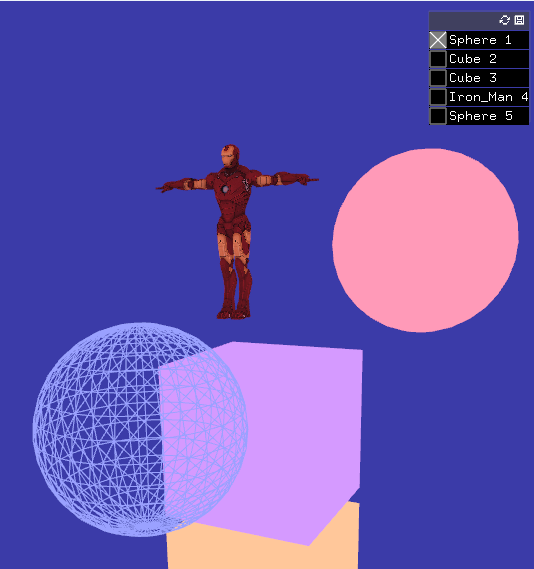
\includegraphics[width=12cm]{fig/WireframeSelection.png}
	\caption{La sélection est en «wireframe»}
	\label{fig:avantTransformation}
\end{figure}

\newpage

Les transformations géométriques peuvent être appliquées en même temps à toutes les entités sélectionnées, en appliquant une matrice de transformation à chacun d'entre eux en même temps. Cette matrice est créée à partir de "sliders", de translation, de rotation et de taille.

\begin{figure}[h]
	\centering
	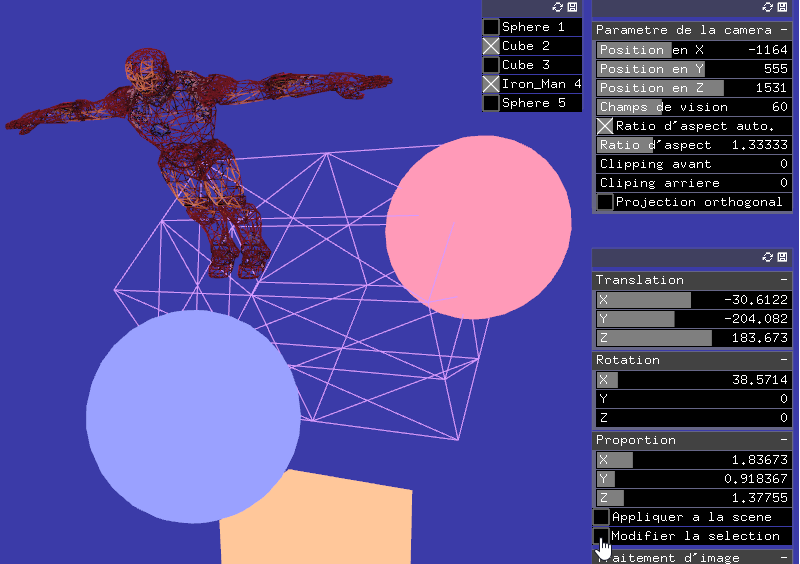
\includegraphics[width=18cm]{fig/transformationSelection.png}
	\caption{Chaque entité de la sélection reçoit la transformation}
	\label{fig:apresTransformation}
\end{figure}

\begin{lstlisting}

void renderer::applySelection(ofMatrix4x4 matrix)
{
	for (auto& p : *scn)
	{
		if (p.selected.get())
		{
			ofMatrix4x4 oldMat = p.getTransfo();
			p.setTransfo(oldMat * matrix);
		}
	}
	std::list<extModel>::iterator iterator4;
	for (iterator4 = externalModels.begin(); iterator4 != externalModels.end(); ++iterator4)
	{
		if (iterator4->selected.get())
		{
			ofMatrix4x4 oldMat = iterator4->getTransfo();
			iterator4->setTransfo(oldMat * matrix);
		}
	}
}
\end{lstlisting}

\begin{lstlisting}

void primitive3d::draw(bool wireframe) {

	ofPushMatrix();
	ofTranslate(transfoMatrix.getTranslation());
	
	ofSetColor(fillCol);
	
	ofQuaternion rotation = transfoMatrix.getRotate();
	float rotationAmount;
	ofVec3f rotationAngle;
	rotation.getRotate(rotationAmount, rotationAngle);
	
	ofRotate(rotationAmount, rotationAngle.x, rotationAngle.y, rotationAngle.z);
	
	ofScale(transfoMatrix.getScale());
	
	if (wireframe || selected.get())
	prim->drawWireframe();
	else
	prim->drawFaces();
	
	ofPopMatrix();
}

\end{lstlisting}

\subsection{Coordonnées non cartésiennes}
Non-implémenté

\subsection{Historique}
Non-implémenté

\pagebreak
\section{Géométrie}
\subsection{Particules}
Non-implémenté

\newpage

\subsection{Primitives}

Dans notre application, il est possible de créer à partir d'algorithmes seulement plusieurs primitives en 3D. Ces primitives sont le cube, la sphère et le cône. Chaque primitive peut être créée directement avec une position et taille choisie par l'utilisateur, mais ces attributs pourront bien évidemment être modifiés par la suite (voir la section 4.3.3 sur la sélection multiple.).\\

On ne peut pas créer les primitives avec une rotation dès le départ, car ce n'est pas pertinent de donner une rotation à un objet comme un cône, quand il n'y a aucun moyen de savoir quelle est son orientation "sans rotation" avant d'en avoir créé un de toute façon. Il faut leur donner la rotation voulue après les avoir créées.\\

On peut aussi choisir une couleur par primitive, dans l'espace de couleur HSB.

\begin{figure}[h]
	\centering
	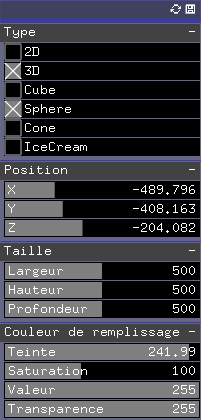
\includegraphics[width=6cm]{fig/creationPrimitive.png}
	\caption{Options de création d'une primitive}
	\label{fig:creationPrimitive}
\end{figure}

\newpage

\begin{lstlisting}
void ofApp::btnDrawPrimitiveClicked()
{
ofLog() << "<app::btnDrawPrimitiveClicked>";

if (primType2D.get()) {
if (primTypeCube.get()) {
selectionMenu.add(rend->createSquare(primPosX, primPosY, primSizeWidth, primSizeHeight));
}
else if (primTypeSphere.get()) {
selectionMenu.add(rend->createCircle(primPosX, primPosY, primSizeWidth, primSizeHeight));
}
else if (primTypeTriangle.get()) {
selectionMenu.add(rend->createTriangle(primPosX, primPosY, primPosX + primSizeWidth, primPosY, (primPosX + primSizeWidth) / 2, primPosY + primSizeHeight));
}
else if (primTypeLine.get()) {
selectionMenu.add(rend->createLine(primPosX, primPosY, primSizeWidth, primSizeHeight));
}
else if (primTypePoint.get()) {
selectionMenu.add(rend->createPoint(primPosX, primPosY, strokeThickness));
}
}
else {
if (primTypeCube.get()) {
selectionMenu.add(rend->createCube(primPosX, primPosY, primPosZ, primSizeWidth, primSizeHeight, primSizeDepth));
}
else if (primTypeSphere.get()) {
selectionMenu.add(rend->createSphere(primPosX, primPosY, primPosZ, primSizeWidth, primSizeHeight, primSizeDepth));
}
else if (primTypeTriangle.get()) {
selectionMenu.add(rend->createCone(primPosX, primPosY, primPosZ, primSizeWidth, primSizeHeight, primSizeDepth));
}
else {
selectionMenu.add(rend->createIcecream(primPosX, primPosY, primPosZ, primSizeWidth, primSizeHeight, primSizeDepth));
}
}
}
\end{lstlisting}

\newpage

\begin{lstlisting}
//-------------3D primitives-----------------------
ofParameter<bool> renderer::createCube(int x, int y, int z, int w, int h, int d)
{
return createCube(x, y, z, w, h, d, fill);
}

ofParameter<bool> renderer::createCube(int x, int y, int z, int w, int h, int d, ofColor fillCol)
{
ofBoxPrimitive* box = new ofBoxPrimitive();

float smallest = min(w, min(h, d));

box->setWidth(smallest);
box->setHeight(smallest);
box->setDepth(smallest);

float newX = (float)w / smallest;
float newY = (float)h / smallest;
float newZ = (float)d / smallest;

ofMatrix4x4 matrix = ofMatrix4x4();
matrix.scale(newX, newY, newZ);
matrix.setTranslation(x, y, z);

for (int i = 0; i < 6; i++)
{
box->setSideColor(i, fillCol);
}

primitive3d prim = primitive3d{ box, fillCol, matrix };
prim.setName("Cube " + to_string(scn->nbElements() + 1));
scn->addElement(prim);
return prim.selected;
}

ofParameter<bool> renderer::createSphere(int x, int y, int z, int sizeX, int sizeY, int sizeZ)
{
return createSphere(x, y, z, sizeX, sizeY, sizeZ, fill);
}

ofParameter<bool> renderer::createSphere(int x, int y, int z, int sizeX, int sizeY, int sizeZ, ofColor color)
{
ofSpherePrimitive* ball = new ofSpherePrimitive();
ball->setPosition(0, 0, 0);

float smallest = min(sizeX, min(sizeY, sizeZ));

ball->setRadius(smallest/2);

float newX = (float)sizeX / smallest;
float newY = (float)sizeY / smallest;
float newZ = (float)sizeZ / smallest;

ofMatrix4x4 matrix = ofMatrix4x4();
matrix.scale(newX, newY, newZ);
matrix.setTranslation(x, y, z);

primitive3d prim = primitive3d{ ball, color, matrix };
prim.setName("Sphere " + to_string(scn->nbElements() + 1));
scn->addElement(prim);
return prim.selected;
}

ofParameter<bool> renderer::createCone(int x, int y, int z, int sizeX, int sizeY, int sizeZ)
{
return createCone(x, y, z, sizeX, sizeY, sizeZ, fill);
}

ofParameter<bool> renderer::createCone(int x, int y, int z, int sizeX, int sizeY, int sizeZ, ofColor color)
{
ofConePrimitive* cone = new ofConePrimitive();
cone->setPosition(0, 0, 0);

float smallest = min(sizeX, sizeZ);
cone->setRadius(smallest / 2);
cone->setHeight(sizeY);

float newX = (float)sizeX / smallest;
float newY = 1.0f;
float newZ = (float)sizeZ / smallest;

ofMatrix4x4 matrix = ofMatrix4x4();
matrix.scale(newX, newY, newZ);
matrix.setTranslation(x, y, z);

primitive3d prim = primitive3d{ cone, color, matrix };
prim.setName("Cone " + to_string(scn->nbElements() + 1));
scn->addElement(prim);
return prim.selected;

}
\end{lstlisting}

\subsection{Modèle}

Il est possible pour un utilisateur d'importer un modèle choisi sur son ordinateur. Les modèles supportés sont ceux qui ont un des formats suivants:

\begin{list}{}{}
	\item 3DS \tab ASE \tab DXF \tab HMP \tab MD2 \tab MD3
	\item MD5 \tab MDC \tab MDL \tab NFF \tab PLY \tab STL 
	\item X \tab LWO \tab OBJ \tab SMD \tab Collada \tab LWO
	\item Ogre XML \tab partly LWS
\end{list}

\begin{figure}[h]
	\centering
	\includegraphics[width=6cm]{fig/importerModele.png}
	\caption{Bouton pour importer un modèle}
	\label{fig:importModel}
\end{figure}

Si le modèle est dans un répertoire avec ses textures dans le bon chemin relatif, celles-ci seront automatiquement chargées et appliquées. De plus, si l'importation du modèle échoue pour une quelconque raison, un message sera affiché à l'utilisateur pour l'informer.\\

Un modèle peut être sélectionné comme une primitive, sera affecté par le mode "Wireframe", et sera modifié si on applique une matrice de transformation pendant qu'il est sélectionné.

Une partie du code qui suit vient de MSDN (Microsoft), dont le lien peut-être trouvé dans la section Références. Nous avons modifié le code pour qu'il convienne à nos besoins.

\begin{lstlisting}
void ofApp::btnImportClicked()
{
HRESULT hr = CoInitializeEx(NULL, COINIT_APARTMENTTHREADED |
COINIT_DISABLE_OLE1DDE);
if (SUCCEEDED(hr))
{
IFileOpenDialog *pFileOpen;

// Create the FileOpenDialog object.
hr = CoCreateInstance(CLSID_FileOpenDialog, NULL, CLSCTX_ALL,
IID_IFileOpenDialog, reinterpret_cast<void**>(&pFileOpen));

if (SUCCEEDED(hr))
{
// Show the Open dialog box.
hr = pFileOpen->Show(NULL);

// Get the file name from the dialog box.
if (SUCCEEDED(hr))
{
IShellItem *pItem;
hr = pFileOpen->GetResult(&pItem);
if (SUCCEEDED(hr))
{
LPWSTR pszFilePath;
hr = pItem->GetDisplayName(SIGDN_FILESYSPATH, &pszFilePath);

// Display the file name to the user.
if (SUCCEEDED(hr))
{

std::wstring path = wstring(pszFilePath);
std::string strPath(path.begin(), path.end());
ofParameter<bool> param = rend->importModel(strPath);

if (param.get() == false)
{
selectionMenu.add(param);
strPath = "Le modele " + strPath + " a ete importe avec succes!";
path = std::wstring(strPath.begin(), strPath.end());
LPCWSTR title = (LPCWSTR)path.c_str();
MessageBox(NULL, title, L"Succes", MB_OK);
}
else
{
strPath = "Le modele n'a pas pu etre importe.";
path = std::wstring(strPath.begin(), strPath.end());
LPCWSTR title = (LPCWSTR)path.c_str();
MessageBox(NULL, title, L"Echec", MB_OK);
}

CoTaskMemFree(pszFilePath);
}
pItem->Release();
}
}
pFileOpen->Release();
}
CoUninitialize();
}
}
\end{lstlisting}

\begin{lstlisting}
ofParameter<bool> renderer::importModel(string path) {
ofxAssimpModelLoader* model = new ofxAssimpModelLoader();
bool ret = model->loadModel(path, false);
if (ret)
{
model->enableTextures();
ofTexture tex = ofTexture();
extModel mod = extModel(model);

string fName(path);
size_t pos = fName.rfind(".");
if (pos != string::npos)
{
if (pos != 0)
{
fName = fName.substr(0, pos);
}
}
pos = fName.rfind("\\");
if (pos != string::npos)
{
if (pos != 0)
{
fName = fName.substr(pos + 1);
}
}

mod.setName(fName + " " + to_string(externalModels.size() + 1));
scn->addElement(mod);
return mod.selected;
}
return ofParameter<bool>(true);
}
\end{lstlisting}

\subsection{Texture}
Non-implémenté

\subsection{Géométrie procédurale}
Non-implémenté

\pagebreak
\section{Caméra}
\subsection{Propriétés de caméra}
Les propriétés de la caméra telle que le champ de vision, le ratio d'aspect ainsi que la distance du plan de clipping avant et arrière. Ils peuvent être modifiés dans l'interface graphique à l'aide de «slider». L'essentiel du code se trouve dans «ccamera::update()».


\begin{lstlisting}
cam->setFov(fov.get());
if (autoRatio.get()) {
cam->setForceAspectRatio(false);
} else {
cam->setAspectRatio(ratio.get());
}
cam->setNearClip(nearClip.get());
cam->setFarClip(farClip.get());
\end{lstlisting}

\begin{figure}[h]
	\centering
	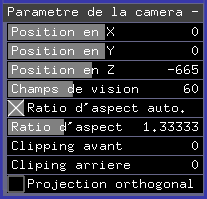
\includegraphics[width=5cm]{fig/proprieteCamera.png}
	\caption{Propriété de la caméra dans l'interface}
	\label{fig:propriete}
\end{figure}

\subsection{Mode de projection}
Le changement de mode de projection de perspective à orthogonale a été implémenté dans l'application. L'essentiel du travail se fait dans la méthode «ccamera::changeMode()». Elle est appelée lorsqu'on appuie sur le bouton à cet effet dans l'interface graphique.

\begin{lstlisting}
if (ortho.get()) {
cam->enableOrtho();
} else {
cam->disableOrtho();
}
\end{lstlisting}

\subsection{Caméra interactive}
La caméra interactive est implémentée dans l'application principalement à l'aide de la classe ofEasyCam de openFrameworks. Nous avons tout de même ajouté la possibilité de déplacer à l'aide des flèches du clavier, pour permettre de repositionner facilement la caméra. Il est aussi possible d'avancer à caméra à l'aide de pageUp/Down. L'essentiel du code se trouve au début de «ccamera::update()».

\begin{lstlisting}
float dist = speed * dt;
float dx = 0;
float dy = 0;
float dz = 0;

dx = 0;
if (isCameraMoveLeft)
dx += dist;
if (isCameraMoveRight)
dx -= dist;
cam->truck(-dx);
posX.set(round(-cam->getX()));

dy = 0;
if (isCameraMoveUp)
dy -= dist;
if (isCameraMoveDown)
dy += dist;
cam->boom(-dy);
posY.set(round(cam->getY()));

dz = 0;
if (isCameraMoveForward)
dz -= dist;
if (isCameraMoveBackward)
dz += dist;
cam->dolly(dz);
posZ.set(round(cam->getZ()));
\end{lstlisting}

\subsection{Caméra multiple}
Non-implémenté

\subsection{Caméra animée}
Non-implémenté


\pagebreak
\section{Pipeline de rendu}
\subsection{Portabilité}
Non-implémenté

\subsection{Shader de géométrie}
Non-implémenté

\subsection{Rétroaction de transformation}
Non-implémenté

\subsection{Passes de rendu}
Non-implémenté

\subsection{Techniques d'occlusion}
Non-implémenté


\pagebreak
\section{Illumination}
\subsection{Types de lumière}
Non-implémenté

\subsection{Lumières multiples}
Non-implémenté

\subsection{Matériaux}
Non-implémenté

\subsection{Modèle d'illumination}
Non-implémenté

\subsection{Volume de lumière}
Non-implémenté


\pagebreak
\section{Lancer de rayon}
\subsection{Intersection}
Dans l'application, il y a des fonctionnalités de lancer de rayon. Celles-ci sont utilisées pour faciliter la sélection d'entités dans la scène. Cette fonctionnalité n'est implementé que pour 2 types de primitives géométriques, soit les cubes et les sphères.

Le fonctionnement est très simple. Comme dans la section 5.3.3 (Sélection multiple), on pouvait ajouter ou retirer des objets de la sélection. Avec le lancer de rayon, tout clic dans la fenêtre lancera un rayon, et si celui-ci intersecte avec une primitive de type cube ou sphère (les seuls supportés), ce agira comme si on avait cliqué sur sa case a coché. Cela l'ajoutera ou le retirera de la sélection courante, selon si cet objet était déjà sélectionné ou pas.

Le rayon n'intersecte pas les objets qui sont derrière la caméras (qui sont pourtant touchés par le rayon qui est infini dans les deux sens) car on ne conserve que les intersections à distance positive vers l'avant. De plus, si plusieurs primitives valides sont en intersection avec le rayon, la selection n'affectera que celle qui est la plus proche de la caméra, puisque logiquement c'est sur celle-ci que l'utilisateur a cliqué, car la partie sous le clic de la seconde primitive est forcément cachée par la première du point de vue de la caméra.

\begin{lstlisting}
struct hit {
	int faceIndex;
	float distance;
};

struct by_distance {
	bool operator()(hit const &a, hit const &b) {
		return a.distance < b.distance;
	}
};
\end{lstlisting}

\begin{lstlisting}
bool primitive::intersectsMesh(ofRay ray, const ofMesh &mesh, const ofMatrix4x4 &toWorldSpace, vector<hit> *meshHit) {
	const vector<ofMeshFace>& faces = mesh.getUniqueFaces();
	bool intersection = false;
	bool intersectedOnce = false;
	vector<hit> distances = vector<hit>();
	for (int i = 0; i < faces.size(); i++) {
		const ofMeshFace &face = faces[i];
		// intersections are done worldSpace
		ofVec3f one = face.getVertex(0) * toWorldSpace;
		ofVec3f two = face.getVertex(1) * toWorldSpace;
		ofVec3f three = face.getVertex(2) * toWorldSpace;
		one = one * transfoMatrix;
		two = two * transfoMatrix;
		three = three * transfoMatrix;
		
		float t;
		intersection = calcTriangleIntersection(one, two, three, ray, &t);
		
		if (intersection && t > 0) {
			hit newHit = hit();
			newHit.distance = t;
			newHit.faceIndex = i;
			distances.push_back(newHit);
			intersectedOnce = true;
			//break;
		}
	}
	
	if (intersectedOnce)
	{
		std::sort(distances.begin(), distances.end(), by_distance());
		for (int i = 0; i < distances.size(); i++)
		{
			meshHit->push_back(distances[i]);
		}
	}
	
	return intersectedOnce;
}

bool primitive::calcTriangleIntersection(const ofVec3f &vert0, const ofVec3f &vert1, const ofVec3f &vert2, ofRay ray, float *result) const
{

	ofVec3f edge1, edge2, tvec, pvec, qvec;
	float det;
	float u, v;
	const float EPSILON = 0.000001f;
	
	edge1 = vert1 - vert0;
	edge2 = vert2 - vert0;
	
	pvec = ray.getTransmissionVector().getNormalized().getCrossed(edge2);
	det = edge1.dot(pvec);
	
	#if 0 // we don't want to backface cull
		if (det < EPSILON)
			return false;
		tvec = getOrigin() - vert0;
		
		u = tvec.dot(pvec);
		if ((u < 0.0f) || (u > det))
			return false;
		
		qvec = tvec.getCrossed(edge1);
		v = getDirection().dot(qvec);
		if (v < 0.0f || u + v > det)
			return false;
		
		*result = edge2.dot(qvec) / det;
		return true;
	#else
		if (det > -EPSILON && det < EPSILON)
			return false;
		
		float inv_det = 1.0f / det;
		tvec = ray.getStart() - vert0;
		u = tvec.dot(pvec) * inv_det;
		if (u < 0.0f || u > 1.0f)
			return false;
		
		qvec = tvec.getCrossed(edge1);
		
		v = ray.getTransmissionVector().getNormalized().dot(qvec) * inv_det;
		if (v < 0.0f || u + v > 1.0f)
			return 0;
		
		*result = edge2.dot(qvec) * inv_det;
		return true;
	#endif
}
\end{lstlisting}

\begin{lstlisting}
vector<hit> primitive3d::intersectsMeshInstance(const ofVec2f &screenCoordinates, const ofCamera &cam) {

	ofMatrix4x4 toWorldSpace = prim->getGlobalTransformMatrix();
	ofMesh mesh = prim->getMesh();
	
	vector<hit>* hits = new vector<hit>();
	
	ofVec3f screenToWorld = cam.screenToWorld(ofVec3f(screenCoordinates.x, screenCoordinates.y, 0.0));
	ofRay ray(cam.getPosition(), screenToWorld - cam.getPosition());
	
	intersectsMesh(ray, mesh, toWorldSpace, hits);
	
	return *hits;
}
\end{lstlisting}

\begin{lstlisting}
void renderer::selectPrimitive(int x, int y, bool shiftHeld)
{
	primitive* toSelect;
	float distance = -1;
	for (primitive& p : *scn)
	{
		vector<hit> hits = p.intersectsMeshInstance(ofVec2f(x, y), (**cam));
		if (hits.size() > 0 && (distance == -1 || hits[0].distance < distance))
		{
			distance = hits[0].distance;
			toSelect = &p;
		}
	}
	
	if (distance > -0.9)
	{
		toSelect->changeSelected();
	}
}
\end{lstlisting}

\begin{lstlisting}
void ofApp::mouseReleased(int x, int y, int button) {
	rend->selectPrimitive(x, y, GetKeyState(VK_SHIFT));
}
\end{lstlisting}

\newpage

\subsection{Réflexion}
Dans notre application, il est possible de créer des cubes de type "miroir".

\begin{figure}[h]
	\centering
	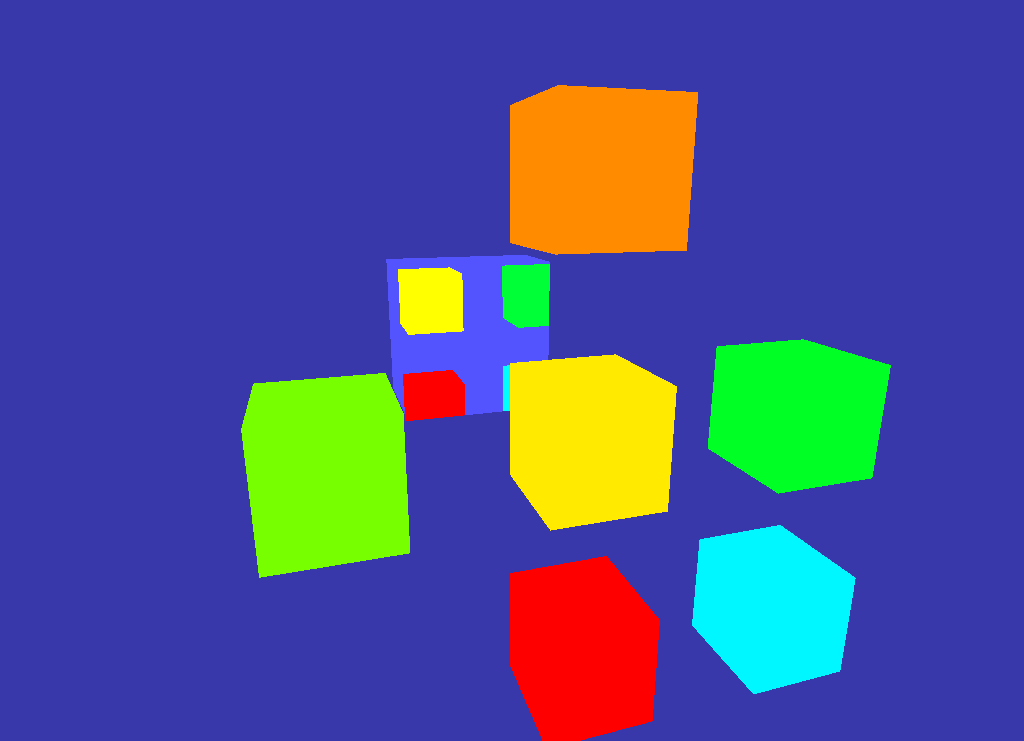
\includegraphics[width=8cm]{fig/CubeReflection1.png}
	\caption{Cube de type miroir}
	\label{fig:propriete}
\end{figure}

\smallskip

Chacune des faces d'un tel cube réflète son entourage. À cause des limitations de temps (et de vitesse de calcul), seuls les sphères et les autres cubes s'affichent dans les miroirs, car, de par le point précédent, ce sont les seuls objets qui incorporent le lancer de rayon.

\begin{figure}[h]
	\centering
	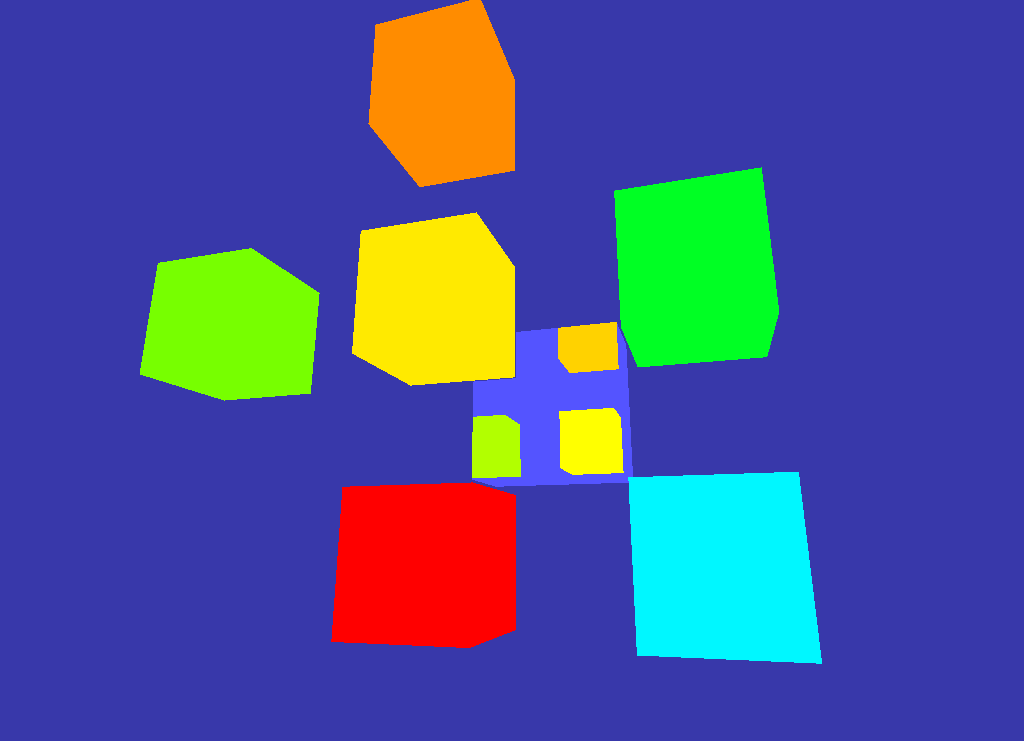
\includegraphics[width=8cm]{fig/CubeReflection2.png}
	\caption{Les miroirs prennent la caméra en compte}
	\label{fig:propriete}
\end{figure}

\smallskip

Tout ce qui est reflété dans un miroir, même le fond de la scène, est rendu un peu plus pâle (à l'exception des pixels déjà blancs, évidemment). Cela est fait pour que les délimitations de la surface miroir soient facile à voir, car sinon elles seraient identiques au fond derrière, et donc partiellement invisible.

\begin{figure}[h]
	\centering
	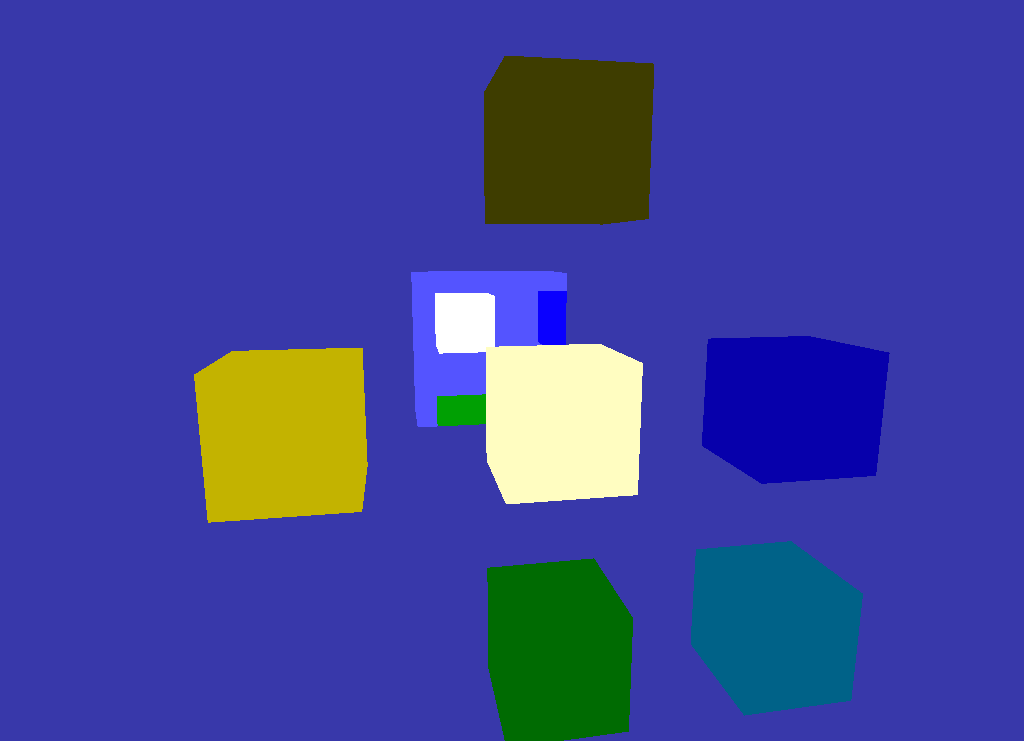
\includegraphics[width=8cm]{fig/CubeReflection3.png}
	\caption{On voit que le fond et chaque cube sont plus pâles que les vrais}
	\label{fig:propriete}
\end{figure}

\begin{figure}[h]
	\centering
	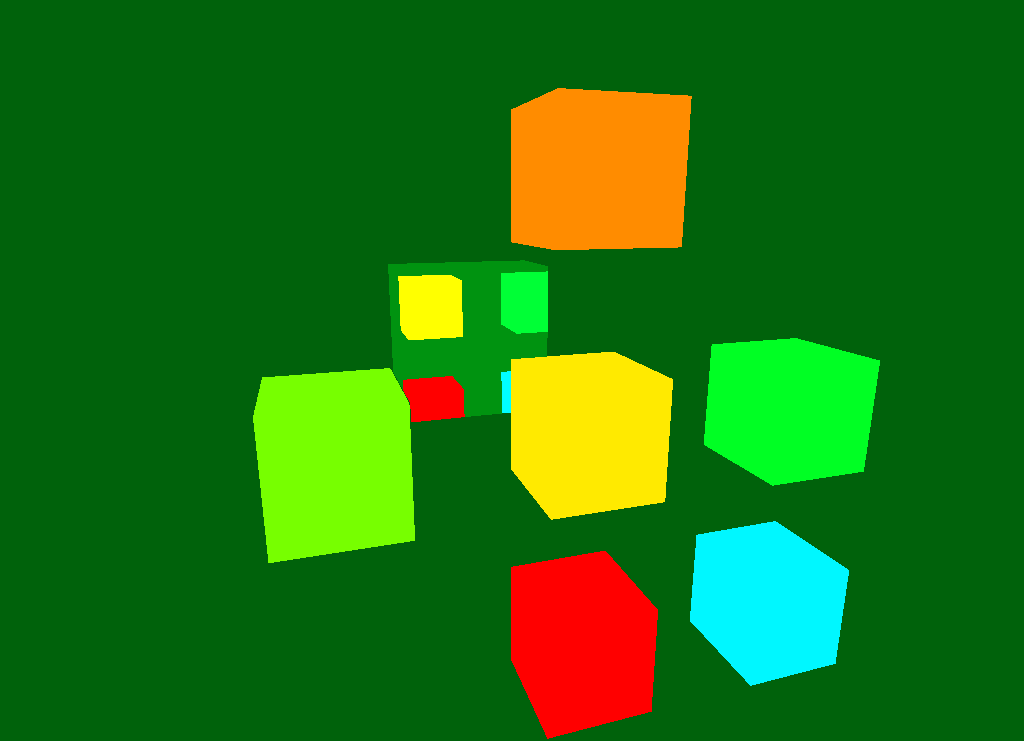
\includegraphics[width=8cm]{fig/CubeReflectionBackground.png}
	\caption{Évidemment, la couleur de fond choisie par l'utilisateur est parfaitement compatible avec les miroirs}
	\label{fig:propriete}
\end{figure}

\smallskip

Il est techniquement aussi possible de créer des sphères miroir, mais nous n'avons pas mis d'option pour le faire dans l'interface.

\smallskip

En effet, la charge de calcul pour les cubes est déjà terriblement élevée, et celle-ci ne fait que grandir très rapidement avec le nombre de triangles du miroir et des entités refletées. Cela fait que, pour un cube ne reflétant que d'autres cubes, cela peut prendre jusqu'à 1 minute pour générer une seule frame. Si le cube doit refléter des sphères, ce temps augmente à plusieurs minutes, et si le miroir est lui-même une sphère, on peut avoir jusqu'à des heures d'attente si le miroir occupe une assez grande partie de l'écran (on envoie un rayon par pixel qui est au dessus d'un miroir après tout). C'est la raison pourquoi nous avons jugé inutile d'offrir l'option des sphères miroirs dans le menu, et nous recommandons fortement de n'utiliser que des cubes pour tester les miroirs.

\smallskip

Pour éviter de complètement geler la fenêtre en permanence parce que chaque frame prend beaucoup de temps à se générer, les miroirs sont configurés en mode "manuel". Cela signifie que L'utilisateur doit spécifier au miroir qu'il veut le rafraichir, et que sinon, le miroir ne se met pas à jour en temps réel.

\begin{figure}[h]
	\centering
	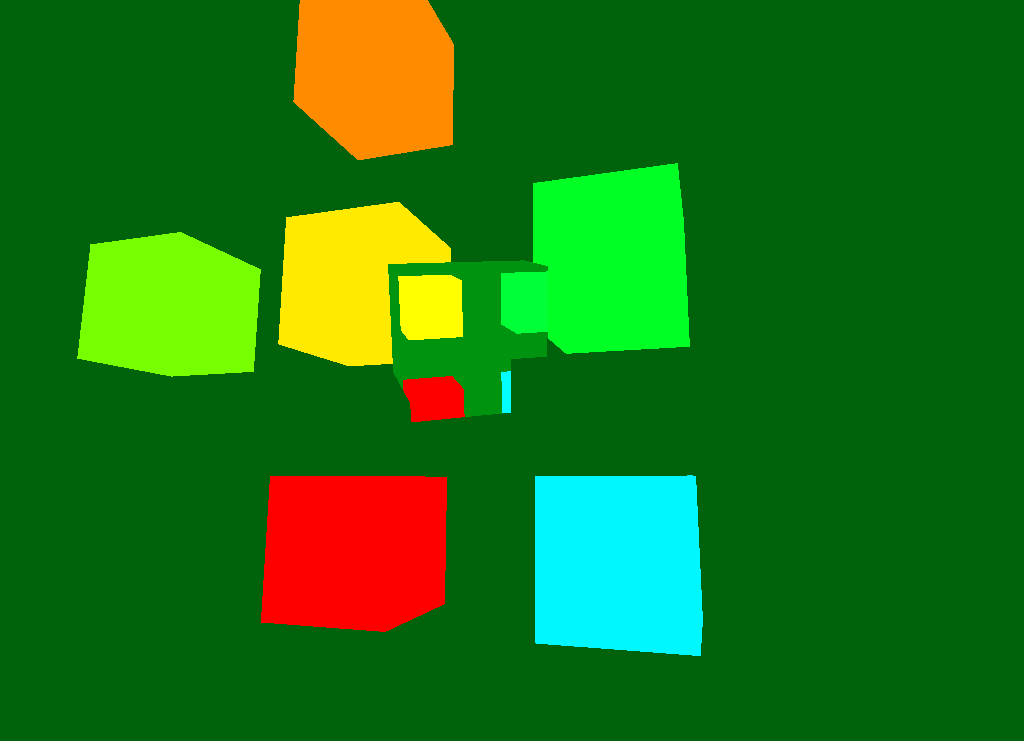
\includegraphics[width=8cm]{fig/CubeReflectionRefreshManuel.png}
	\caption{Après un mouvement de caméra, le miroir ne s'est pas mis à jour à chaque frame, pour éviter des délais de plusieurs minutes}
	\label{fig:propriete}
\end{figure}

\smallskip

Nous avons simplement, pour les besoins du travail, configuré l'événement qui met à jour les miroirs sur le relâchement d'une touche du clavier. L'utilisateur se positionne donc de façon fluide comme il veut, et ensuite il peut appuyer sur la touche de son choix pour démarrer l'attente de 30-60sec pour rendre le miroir avec le nouvel angle.

\begin{figure}[h]
	\centering
	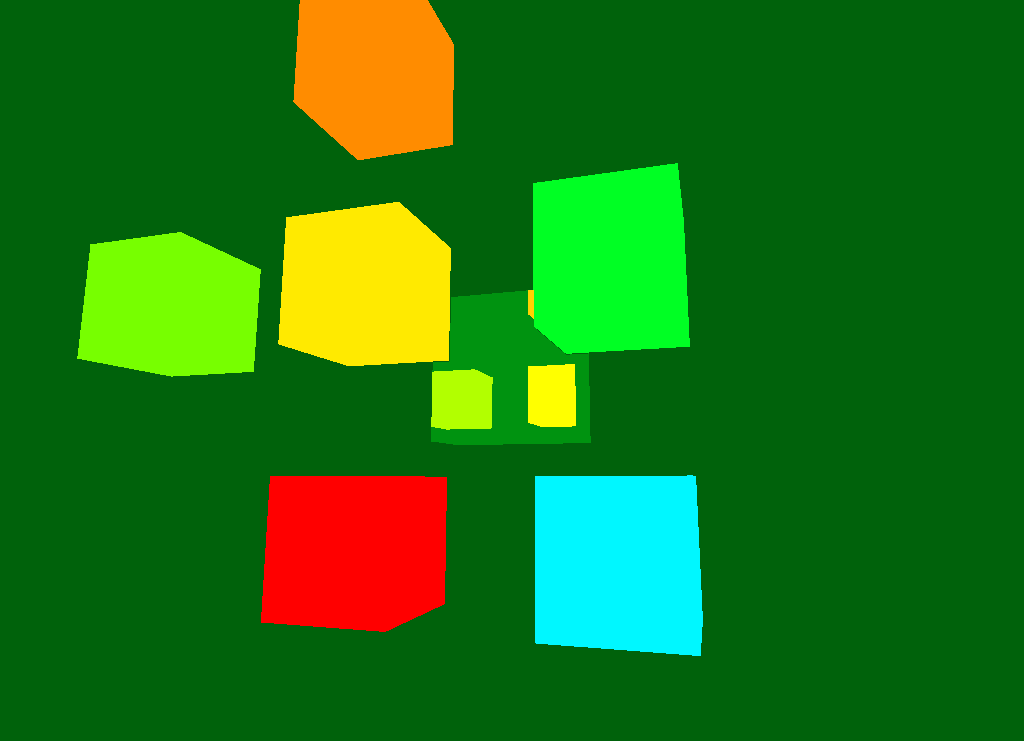
\includegraphics[width=8cm]{fig/CubeReflectionApresRefresh.png}
	\caption{L'utilisateur appuis sur une touche, attend la génération de la frame, et le miroir est maintenant à jour!}
	\label{fig:propriete}
\end{figure}

\bigskip
De plus, les miroirs se mettent à jour une fois à leur première apparition, et automatiquement quand la composition de la scène change (ajout de primitive).

\smallskip

Pour le code: voir la section 5.8.3 Réfraction, car ces deux fonctionnalités ont beaucoup de code en commun, donc pour éviter de l'avoir deux fois, le code sera recopié dans cette section.

\newpage

\subsection{Réfraction}
Comme pour la réflection, notre application permet la réfraction sur les primitives de type cube, et on ne voit dans les objets avec réfraction que les cubes et les sphères. Les délais de calculs sont aussi très longs, donc les mêmes limitations s'appliquent, incluant la mise à jour manuelle des surfaces avec réfraction.

\begin{figure}[h]
	\centering
	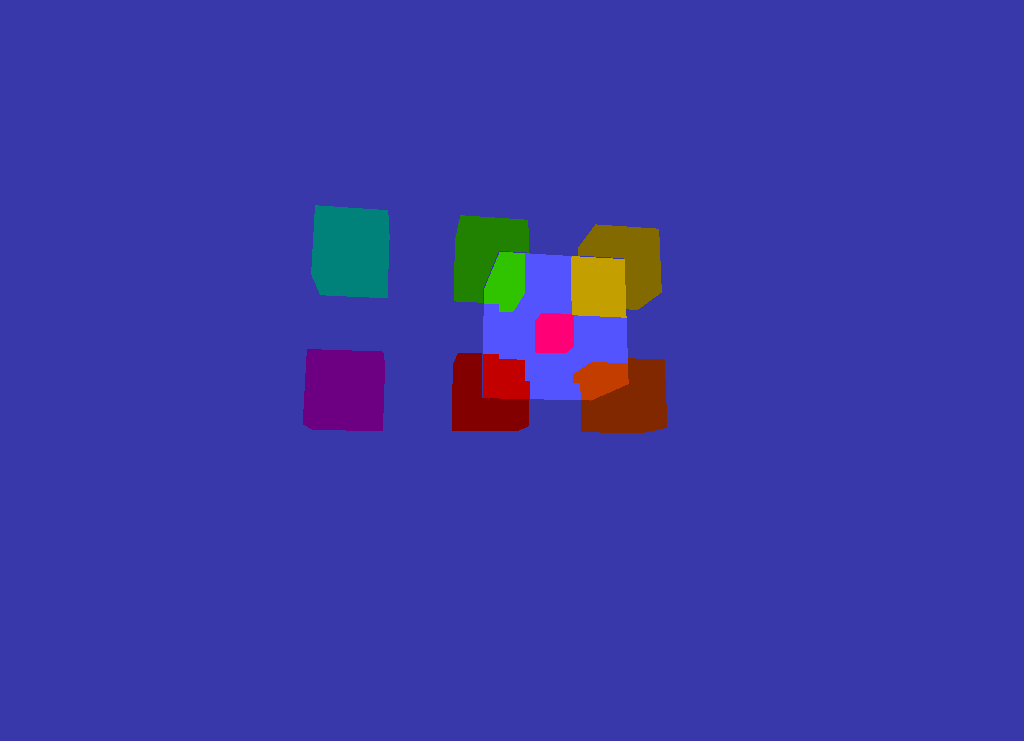
\includegraphics[width=8cm]{fig/CubeRefraction.png}
	\caption{Un cube de vitre distortionne un peu la lumière, et donc les objets derrière sont un peu changés selon au travers de quelle face du cube on les regarde}
	\label{fig:propriete}
\end{figure}

\smallskip

Comme cette fonctionnalité est littéralement une réflexion dont le rayon incident est calculé d'une autre façon, on a exactement le meme comportement dans toutes situations, incluant rendre les objets visibles à l'intérieur plus pâles, et un support de la couleur de fond de la scène. Encore une fois, les primitives et objets autre que "Cube" et "Sphère" seront invisible par réfraction, et les sphères ralentissent considérablement le temps (déjà long) de génération d'une image.

Code (incluant le code de réflexion):

\begin{lstlisting}
void renderer::draw()
{
	vector<primitive*> GlassyPrims;
	vector<primitive*> other3D;
	
	for (auto& p : *scn)
	{
		if (p.isCubeOrSphere()) // Inutile d'essayer de "voir" les autres types, puisqu'ils ne sont pas implementes.
		{
			other3D.push_back(&p);
			if (p.isGlassy()) // Une primitive "glassy" est soit un miroir, soit une vitre avec refraction
			{
				GlassyPrims.push_back(&p);
			}
		}
	}
	
	ofClear(background);
	
	cam->begin();
	ofPushMatrix();
	
	ofEnableDepthTest();
	//ofEnableLighting();
	
	ofSetLineWidth(1.0);
	
	if (translate) {
		ofTranslate(deltaX, deltaY, deltaZ);
	}
	if (rotate) {
		ofRotate(centerX, 1, 0, 0);
		ofRotate(centerY, 0, 1, 0);
		ofRotate(centerZ, 0, 0, 1);
	}
	if (scale) {
		ofScale(scaleX, scaleY, scaleZ);
	}
	
	for (auto& p : *scn)
	{
		p.draw(wireFrame, lightShader);
	}
	
	std::list<ofRay>::iterator iterator2;
	bool origRay = true;
	for (iterator2 = rays.begin(); iterator2 != rays.end(); ++iterator2)
	{
		if (origRay)
			ofSetColor(255, 0, 0);
		else
			ofSetColor(0, 255, 0);
		iterator2->draw();
		origRay = !origRay;
	}
	
	//ofDisableLighting();
	ofDisableDepthTest();
	
	ofPopMatrix();
	
	cam->end();
	
	for (auto& glassy : GlassyPrims) // Toutes les primitives "glassy"
	{
		vector<ofRay> newRays = glassy->prepareGlass((**cam), other3D, background); // On les prepare
		for (auto r : newRays)
		{
			//rays.push_back(r); // A des fins de debogage, on peut faire afficher une partie des rayons de lumiere, pour voir leur comportement
		}
	}
	
	if (isFiltered) {
		checkFilters();
	}
}
\end{lstlisting}

\begin{lstlisting}
// Permet d'obtenir la couleur de la primitive Si et seulement si elle est touchee par un rayon
bool primitive3d::getColorOfRay(ofRay ray, ofColor * colHit) {
	ofMatrix4x4 toWorldSpace = prim->getGlobalTransformMatrix();
	ofMesh mesh = prim->getMesh();
	
	vector<hit>* hits = new vector<hit>();
	
	vector<ofMeshFace> allFaces = mesh.getUniqueFaces();
	
	bool hasHit = intersectsMesh(ray, mesh, toWorldSpace, hits);
	
	if (hasHit)
	{
		//*hit = allFaces[(*hits)[0]].getColor(0);
		*colHit = fillCol;
	}
	return hasHit;
}
\end{lstlisting}

\begin{lstlisting}
// Rend une couleur plus pale, pour eviter les miroirs invisibles
ofColor getSlightlyLighterColor(ofColor original, float ratio = 1.5) {
	int red = original.r;
	int green = original.g;
	int blue = original.b;
	
	red = red * ratio;
	green = green * ratio;
	blue = blue * ratio;
	
	int maxColorValue = ofColor::limit();
	
	// Evidemment, si une des composantes depasse la limite, on la ramene au maximum.
	// On est pas Tide(tm), on ne veut pas que les choses soient plus blanc que blanc!
	if (red > maxColorValue)
		red = maxColorValue;
	if (green > maxColorValue)
		green = maxColorValue;
	if (blue > maxColorValue)
		blue = maxColorValue;
	
	return ofColor(red, green, blue);
}
\end{lstlisting}

\begin{lstlisting}
// Preparation de la vitre/miroir, seulement si necessaire
vector<ofRay> primitive3d::prepareGlass(const ofCamera cam, vector<primitive*> otherPrims, ofColor backgroundCol) {//, const scene * scn) {
	vector<ofRay> returnVec = vector<ofRay>();
	int wid = ofGetWidth();
	int hei = ofGetHeight();
	
	// Si la primitive n'est ni un miroir ni une vitre, on n'a pas notre place ici!
	if (isMirror || isGlass)
	{	
		// Un miroir n'a pas besoin de couleur!
		fillCol = ofColor(255, 255, 255, 0);
		
		// Si un rafraichissement manuel a ete demande depuis la derniere fois.
		if (mustPrepare) {
		
			// matrice de transformation globale
			ofMatrix4x4 toWorldSpace = prim->getGlobalTransformMatrix();
			
			// Le mesh de la primitive
			ofMesh * mesh = prim->getMeshPtr();
			
			// Et ses faces
			vector<ofMeshFace> allFaces = mesh->getUniqueFaces();
			
			int firstX = wid;
			int lastX = 0;
			int firstY = hei;
			int lastY = 0;
			
			// Ca ne sert a rien d'envoyer des rayons sur des pixels qui n'ont aucune chance de toucher la primitive.
			// A des fins d'optimisation, on detecte les limites (en x et y) du rectangle qui contient la primitive, pour ne tester que ces rayons.
			for (int i = 0; i < allFaces.size(); i++) {
				for (int j = 0; j < 3; j++)
				{
					ofVec3f screen = cam.worldToScreen(allFaces[i].getVertex(j) * toWorldSpace * transfoMatrix);
					if (firstX > screen.x)
						firstX = screen.x;
					if (firstY > screen.y)
						firstY = screen.y;
					if (lastX < screen.x)
						lastX = screen.x;
					if (lastY < screen.y)
						lastY = screen.y;
				}
			}
			
			// On ne lance pas de rayon en dehors de l'ecran, voyons. tss tss.
			if (firstX < 0)
				firstX = 0;
			if (firstY < 0)
				firstY = 0;
			if (lastX >= wid)
				lastX = wid - 1;
			if (lastY >= hei - 1)
				lastY = hei;
			
			toPaint = ofImage();
			toPaint.allocate(wid, hei, OF_IMAGE_COLOR_ALPHA);
			
			for (int i = 0; i < wid; i++)
			{
				for (int j = 0; j < hei; j++)
				{
					toPaint.getPixels().setColor(i, j, ofColor(255, 255, 255, 0));
				}
			}
			
			allFaces = mesh->getUniqueFaces();
			
			// Dans notre rectangle, feu a volonte!
			for (int x = firstX; x <= lastX; x++)
			{
				for (int y = firstY; y <= lastY; y++)
				{
				
					ofVec3f screenToWorld = cam.screenToWorld(ofVec3f(x, y, 0.0));
					ofRay ray(cam.getPosition(), screenToWorld - cam.getPosition());
					
					ofVec2f coords = ofVec2f(x, y);
					
					primitive* toSelect;
					float distance = -1;
					vector<hit> hits;
					vector<hit> realHits;
					
					// On lance un rayon sur chaque pixel en cherchant si il intersecte notre miroir.
					for (auto& otherPrim3D : otherPrims)
					{
						hits = (otherPrim3D->intersectsMeshInstance(coords, cam));;
						if (hits.size() > 0 && (distance == -1 || (hits)[0].distance < distance))
						{
							distance = (hits)[0].distance;
							toSelect = otherPrim3D;
							realHits = hits;
						}
					}
					
					// Si on a intersecte notre miroir/vitre, ET qu'on a rien intersecte de plus proche avec le meme rayon, on peut travailler.
					if (distance > -0.9 && toSelect->getName() == getName()) {
						// La face touchee
						const ofMeshFace * face = &allFaces[(realHits)[0].faceIndex];
						
						ofColor col = backgroundCol;
						
						ofRay mathReflectedRay = ofRay();
						
						if (isMirror) {
							// Les sommets du triangle touche
							ofVec3f A = face->getVertex(0) * toWorldSpace;
							ofVec3f B = face->getVertex(1) * toWorldSpace;
							ofVec3f C = face->getVertex(2) * toWorldSpace;
							
							A = A * transfoMatrix;
							B = B * transfoMatrix;
							C = C * transfoMatrix;
							
							// Des maths. Sont assez self-explanatory pour ceux qui connaissent ca, et prendraient des dizaines de lignes de commentaires a expliquer sinon.
							// Good luck!
							ofVec3f AB = B - A;
							ofVec3f AC = C - A;
							
							ofVec3f ABxAC = AB.getCrossed(AC);
							
							ofVec3f n = (ABxAC) / (ABxAC.length());
							ofVec3f v = ray.getTransmissionVector();
							
							ofVec3f OK = (v.dot(n)) * n;
							ofVec3f OL = 2 * OK;
							
							ofVec3f w = v - OL;
							
							ofVec3f S = ray.getStart();
							ofVec3f SA = (A - S);
							
							float t = (n.dot(SA)) / (n.dot(v));
							
							ofVec3f OR = S + (t * v);
							
							// Juste pour que le rayon soit visible (mais pas infini) quand on l'affiche pour deboguer
							w = w.scale(1000);
							
							// Long story short, on a trouve l'origine et la direction du rayon reflete, donc c'est cool
							mathReflectedRay = ofRay(OR, w, false);
						}
						else if (isGlass)
						{
						
							// Si on est une vitre, on fait sensiblement la meme chose
							ofVec3f A = face->getVertex(0) * toWorldSpace;
							ofVec3f B = face->getVertex(1) * toWorldSpace;
							ofVec3f C = face->getVertex(2) * toWorldSpace;
							
							A = A * transfoMatrix;
							B = B * transfoMatrix;
							C = C * transfoMatrix;
							
							ofVec3f AB = B - A;
							ofVec3f AC = C - A;
							
							ofVec3f ABxAC = AB.getCrossed(AC);
							
							ofVec3f n = (ABxAC) / (ABxAC.length());
							ofVec3f invN = -n;
							ofVec3f v = ray.getTransmissionVector();
							
							// Sauf ici.
							ofVec3f w = ofVec3f((v.x + n.x) / 2, (v.y + n.y) / 2, (v.z + n.z) / 2);
							
							ofVec3f S = ray.getStart();
							ofVec3f SA = (A - S);
							
							float t = (n.dot(SA)) / (n.dot(v));
							
							ofVec3f OR = S + (t * v);
							
							w = w.scale(1000);
							
							// Basically, on part vers l'interieur plutot que vers l'exterieur, et on genere encore le beau rayon tout neuf.
							mathReflectedRay = ofRay(OR, w, false);
						}
						
						// Si on veut deboguer les rayons, tous les afficher serait un mechant desordre. On en affiche donc seulement 1/800, choisis au hasard, ca nous en laisse assez pour voir les problemes, mais pas trop pour comprendre leur comportement.
						if (rand() % 800 == 0)
						{
							ray.color = ofColor(255, 0, 0);
							mathReflectedRay.color = ofColor(0, 255, 0);
							returnVec.push_back(ray);
							returnVec.push_back(mathReflectedRay);
						}
						
						// Avec notre nouveau rayon, on va chercher la premiere couleur qu'il touche!
						// Si personne le touche, on se retrouve avec la couleur de fond, car on avait initialise col a ca.
						for (auto& otherPrim3D : otherPrims)
						{
							if (otherPrim3D->getName() != getName())
							{
								otherPrim3D->getColorOfRay(mathReflectedRay, &col);
							}
						}
						
						// Un peu plus pale, les miroirs invisibles c'est villain. On fonce dedans comme un moineau dans une porte patio,
						ofColor lighter = getSlightlyLighterColor(col);
						
						toPaint.getPixels().setColor(x, y, lighter);
					}
				}
			}
			
			// Pas besoin de rafraichir avant de se le faire redemander!
			mustPrepare = false;
		}
	}
	
	// On dessine par dessus le cube notre belle reflexion pas du tout pixelisee. Toute qu'une oeuvre d'art!
	toPaint.update();
	ofSetColor(255);
	toPaint.draw(0, 0, wid, hei);
	
	// Ah et on retourne un rayon sur 800, si jamais le renderer voulait les avoir pour deboguer.
	return returnVec;
}
\end{lstlisting}

\newpage

\subsection{Ombrage}
Non-implémenté

\newpage

\subsection{Rendu graphique}
Non-implémenté

\pagebreak
\section{Topologie}
\subsection{Courbe cubique}
Non-implémenté

\subsection{Courbe paramétrique}
Non-implémenté

\subsection{Surface paramétrique}
Non-implémenté

\subsection{Shader de tesselation}
Non-implémenté

\subsection{Triangulation}
Non-implémenté


\pagebreak
\section{Techniques de rendu}
\subsection{Effet de relief}
Non-implémenté

\subsection{Cube de réflexion}
Non-implémenté

\subsection{BRDF}
Non-implémenté

\subsection{Effet en pleine fenêtre}
Non-implémenté

\subsection{Style libre}
Non-implémenté

